\chapter{Tire Models}

\label{sec:TireModels}
\setcounter{figure}{0}
\setcounter{table}{0}

Currently, nine tire models are implemented in OptimumTire:
\begin{itemize}
\item	Fiala Model
\item	Brush Model
\item Harty Model
\item	Pacejka Magic Formula '96 Model
\item	Pacejka Magic Formula 2002 Model
\item	Pacejka Magic Formula 2002 Model with Inflation Pressure effects
\item	Pacejka Magic Formula 2006 Model
\item	Magic Formula 5.2 Model
\item	Magic Formula 6.1 Model
\end{itemize}

The coefficients of these tire models can be manually inputted or imported from an OptimumTire Native File. OptimumTire can also fit these models to raw tire data. More specific information regarding the tire models is included in the section~\ref{sec:References}.

\section{Manually Input Model}
\label{sec:ManuallyInputModel}
If the tire model coefficients have already been determined, they can be manually inputted into OptimumTire. First select the \textsl{New Tire Model} button at the top of the project tree. Then choose the type of tire model you would like to add to the project. This tire model will be added to the project tree. Right clicking on the tire model allows the user to rename, delete, or copy the model as well as many other functions.
The model coefficients can now be entered into the model input form, which appears in the data entry area when the model is clicked on. An example of this form is shown in Figure~\ref{fig:TireModelForm}. For coefficients that have units the units can be specified in the dropdown boxes to the right of the value. The small plus and minus buttons also to the right of the values allow the user to adjust the model. This feature is covered in detail in section~\ref{sec:AdjustingModels}.

 \begin{figure}[H]
	\centering
		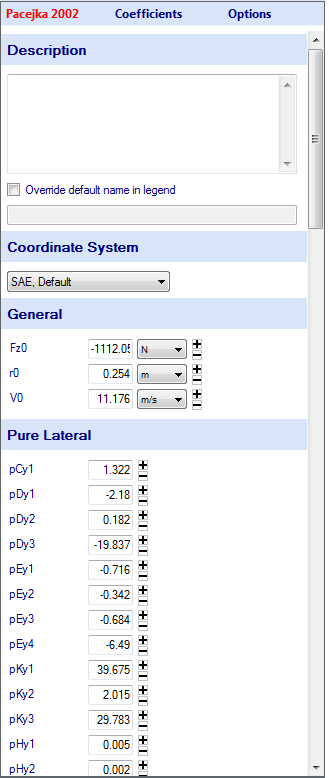
\includegraphics[height=0.95\textheight]{TireModelForm.png}
	\caption{Tire Model Input Form}
	\label{fig:TireModelForm}
\end{figure}

\section{Import and Export Models}
\label{sec:ImportandExportModels}
Before a tire model is imported into OptimumTire the appropriate tire model needs to be added to the project. This is done by clicking on the \textsl{New Tire Model} button at the top of the tire project tree. Once the tire model is added clicking on it will display its coefficients in the data entry area. Since it is a new model all of the coefficients will be zero. At the top of the data entry area click on Options-Import as shown in Figure~\ref{fig:ImportTireModel}. Tire model coefficients can then be imported from an OptimumTire Native file or from a TIR, or similar, file. Note that when you import a model, OptimumTire will overwrite the data contained in the model input form.
 


 \begin{figure}[H]
	\centering
		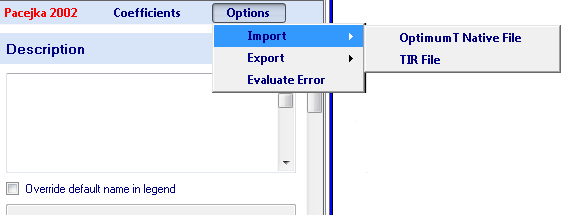
\includegraphics[width=1.0\textwidth]{ImportTireModel.png}
	\caption{Import Tire Model}
	\label{fig:ImportTireModel}
\end{figure}

Tire models can also be exported from OptimumTire by clicking on the desired tire model in the project tree. Then, at the top of the data entry area, click on \textsl{Options-Export} and select the file format you prefer. You can export to OptimumTire Native files, Excel, Lookup tables and into text-based files, such as TIR files. You also have the option of copying the tire model to the clip board for use with the addin (it will be in an encoded text format).

\begin{figure}[H]
	\centering
		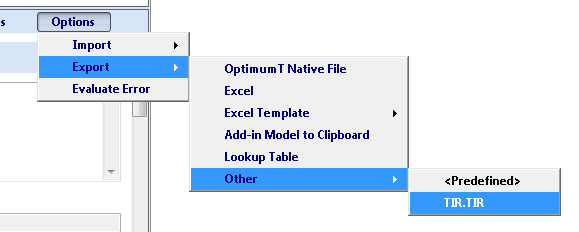
\includegraphics[width=1.0\textwidth]{ExportModel.png}
	\caption{Export Tire Model}
	\label{fig:ExportModel}
\end{figure}


\subsection{Export Templates}
\label{sec:ImportandExportModelsExportTemplate}
When exporting to a text-based format format, like a TIR file, OptimumTire uses export templates. You can edit the export templates in the template manager. When creating a new template, it is recommended that you start with an existing template and modify it. (If you start from a Predefined template, you will need to clone it first because these are read-only). When OptimumTire reads a template, it looks for parameter fields in the format \texttt{\#PARAM\#DEFAULT-VALUE\#}. Note that there are a total of three \texttt{\#} symbols for each parameter. \texttt{PARAM} denotes the name of the parameter, \texttt{DEFAULT-VALUE} denotes the default value for this parameter if it is not found in the tire model. If there are parameters specified in the export template that are not in the tire model, the user will be asked to specify them in a dialog when exporting a model. The default value will be used if the user does not specify a different value when exporting. The model description and coordinate system can be exported using the tags \texttt{\#DESC\#} and \texttt{\#COORDSYS\#} respectively.

When exporting models using templates be aware that the simulation program you intend to use the model with may require the model in a specific coordinate system. Tir and similar files do not contain coordinate system information so the coordinate system must be modified within OptimumTire before exporting. In the case of the MF5.2 and P96 templates, which have been designed for use in RaceSim, you can not export using the SAE coordinate system. It is recommended that you export using the Iso coordinate system for these models.

OptimumTire also offers the ability to export lookup tables for simulation programs that do not directly import model coefficients or equations. For more details on how to use this feature of OptimumTire see section~\ref{sec:LookupTableExport}.

\subsection{Excel Export Templates}
\label{sec:ExcelExportTemplate}
OptimumTire can also export to Microsoft Excel using export templates similar to those explained in the previous section ~\ref{sec:ModelFittingOrder}. An Excel template is a regular Excel worksheet with cells that contain text that can be recognised by OptimumTire. When OptimumTire reads an Excel template it looks for parameter fields in the format \texttt{\#PARAM\#} where PARAM is the name of the coefficient to be exported, eg. pCy1 as shown in Figure ~\ref{fig:ExcelTemplate}. The model description and coordinate system can be exported using the tags \texttt{\#DESC\#} and \texttt{\#COORDSYS\#} respectively (Note OptimumTire will only search the first worksheet of an Excel template for the parameter fields). Once the template has been created the file should be copied and pasted into the application data folder using the template manager or saved in the application data folder:

Windows Vista and Windows 7:\\
\texttt{C:\textbackslash Users\textbackslash UserName\textbackslash AppData\textbackslash Roaming\textbackslash OptimumT\textbackslash ExcelTemplates}

Windows XP:\\
\texttt{C:\textbackslash Documents and Settings\textbackslash UserName\textbackslash Application Data\textbackslash Roaming\textbackslash OptimumT\textbackslash ExcelTemplates}


\begin{figure}[H]
	\centering
		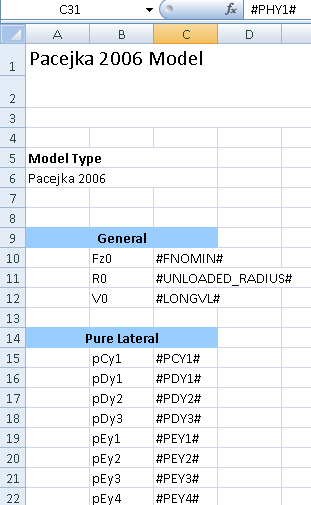
\includegraphics[width=0.5\textwidth]{ExcelTemplate.png}
	\caption{Example Excel Export Template}
	\label{fig:ExcelTemplate}
\end{figure}

\section{Fitting Models to Raw Data}
\label{sec:FittingModelstoRawData}
Before fitting a tire model to the raw data the data should be properly cropped and collapsed. This will make the fitting more accurate and significantly quicker. Also make sure that the \textsl{Use Collapsed Data} option is selected for the tire data that will be used. This can be found at the top of the \textsl{Collapse Data} section in the tire data input area.
The following sections demonstrate how to fit a tire model. This example will use pure lateral and combined longitudinal and lateral data to create a complete tire model. Depending on the data available and the goal of the model fitting the order in which the models are fit can vary. More information about the order the models should be fit is included in section~\ref{sec:ModelFittingOrder}.

\subsection{Pure Lateral Model}
\label{sec:PureLateralModel}
Fitting of the cornering data to the model lateral force coefficients is generally done first. To begin select the tire data to be modeled in the project tree. Go to the last section of the data entry area, labeled \textsl{Model Fitting}. This is shown in Figure~\ref{fig:TireModelSelection}. In the drop down box select the type of tire model to be fitted. Once you have selected the type of model to be used click the \textsl{Fit Model} button. This will open the Model Fitting Tool as can be seen in Figure~\ref{fig:ModelFittingSelection}. 

 \begin{figure}[H]
	\centering
		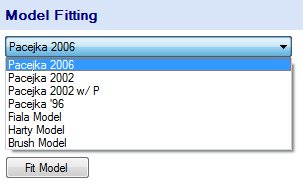
\includegraphics{TireModelSelection.png}
	\caption{Selecting the Tire Model to be Fit}
	\label{fig:TireModelSelection}
\end{figure}

\subsection*{Specify Coefficients to be Calculated}
In the \textsl{Model Fitting Selection} window the coefficients to be fit are selected. The coefficients that the error calculation is based on are also selected by choosing the \textsl{Fit and Calculate Error} option in the dropdown boxes.  For this case you would select \textsl{Fit and Calculate Error} in the drop down box labeled Fy Pure as is shown in Figure~\ref{fig:ModelFittingSelection}. \textsl{Fit and Calculate Error} must always be selected for at least one of the sets of coefficients. At the bottom of this window the coordinate system of the model can be selected.  To proceed click the Next button.

 \begin{figure}[H]
	\centering
		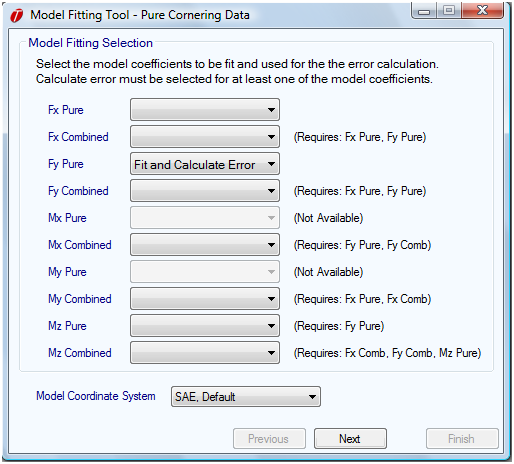
\includegraphics{ModelFittingSelection.png}
	\caption{Model Fitting Selection}
	\label{fig:ModelFittingSelection}
\end{figure}

\subsection*{Model Constraints}
Now the model constraints must be set. The constraints required vary depending on what type of model is being fit. For the Pacejka models the constraints include the nominal (rated) tire load, $F_{z0}$, the unloaded tire radius, $R_0$, the reference velocity, $V_0$, and the reference pressure, $P_0$. Typically the nominal load is set to the largest or second largest load that the tire was tested at, the reference velocity is set to the test velocity, and the reference pressure is set to the highest inflation pressure the tire was tested at. More information regarding these parameters is included in section~\ref{sec:References}.

 \begin{figure}[H]
	\centering
		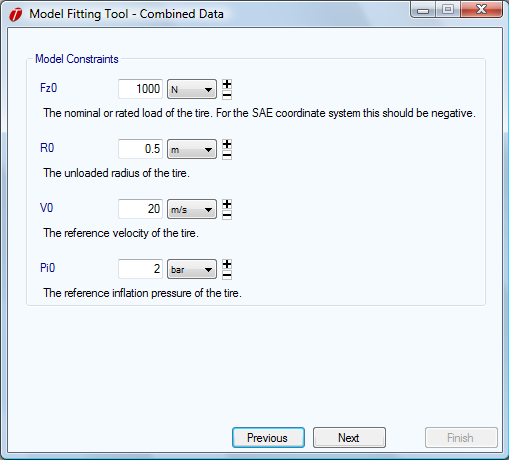
\includegraphics[width=1.0\textwidth]{Constraints.png}
	\caption{Model Constraints}
	\label{fig:Constraints}
\end{figure}

\subsection*{Define the Coefficient Boundary}
Now the \textsl{Coefficient Boundary} to be used in the fitting must be set. The coefficient boundary allows the solver to begin fitting the model in a restricted, more accurate range of values for the coefficients. However, the solver is not necessarily restricted to the range of coefficients set by the boundaries.  In Figure~\ref{fig:CoefficientBoundaries} the Coefficient Boundary window is shown. A \textsl{Coefficient Boundary} is chosen by selecting it from the list. Click on \textsl{Next} to proceed.

\begin{figure}[H]
	\centering
		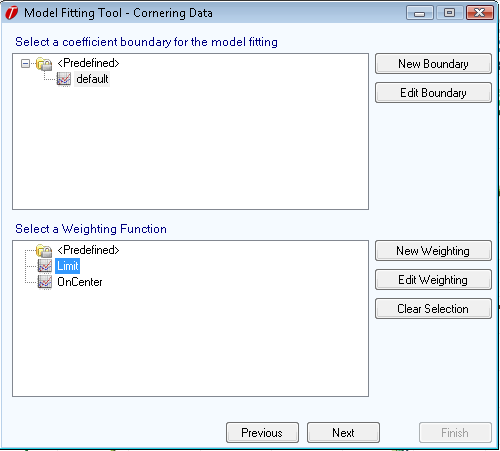
\includegraphics[width=1.0\textwidth]{CoefficientBoundaries.png}
	\caption{Coefficient Boundary}
	\label{fig:CoefficientBoundaries}
\end{figure}

Coefficient boundaries can easily be created or edited by clicking on the \textsl{New Boundary} and \textsl{Edit Boundary} buttons to the right. However the coefficients in the \textsl{Predefined Folder} cannot be modified. If they are edited, the edited version will be saved outside of the \textsl{Predefined} folder and the original version will stay unchanged.  When these buttons are clicked the \textsl{Coefficient Boundary Editor} window will open as shown in Figure~\ref{fig:NewCoefficientBoundary}. This window allows the boundaries for each coefficient to be changed. If the \textsl{Hard Boundary} check boxes are selected the solver will be restricted to finding a solution within this range of coefficients. Save the new or edited boundary by typing in a name at the top of the window and clicking on save. Now you can close this window and the new boundary will be available for selection in the \textsl{Coefficient Boundary} window.

\begin{figure}[H]
	\centering
		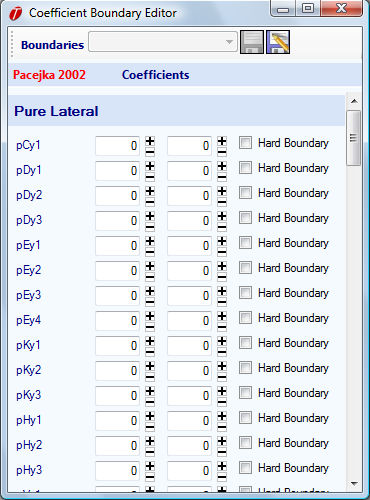
\includegraphics{NewCoefficientBoundary.png}
	\caption{Coefficient Boundary Editor}
	\label{fig:NewCoefficientBoundary}
\end{figure}


\subsection*{Weighting Functions}
Optionally, you can select a weighting function to apply to the fit. This will change the way the error is evaluated. For details about the error evaluation, please see Section \ref{sec:models:solverparameters}. You can select an existing weighting function by selecting it from the list in the coefficient boundary selection dialog (Figure \ref{fig:CoefficientBoundaries}). You can also create a new weighting function or edit an existing one in this dialog. If you have selected a weighting function and wish to remove this selection, click the \textit{Clear Selection} button.

\begin{figure}[H]
	\centering
		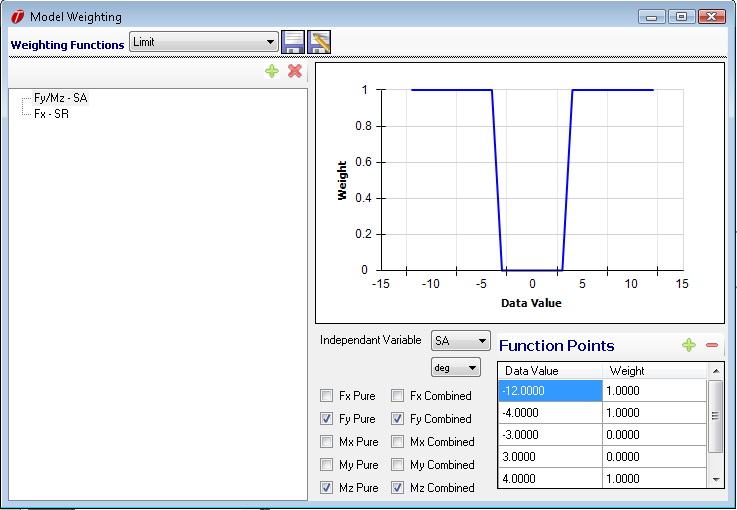
\includegraphics[width=0.90\textwidth]{WeightingFunction.png}
	\caption{The weighting function editor}
	\label{fig:WeightingFunction}
\end{figure}

Figure \ref{fig:WeightingFunction} shows the weighting function editor. It is accessible by clicking either the \textit{New Weighting} or \textit{Edit Weighting} button. At the very top of the dialog, you can save or load a weighting function. On the left side, you can select the \textit{Weighting Pages} which define a part of a weighting function. There is no limit to the number of weighting pages that you can add (though there is a practical limit of 60, as it is not possible to define more than 60 non-redundant weighting pages). Each weighting page has one independent variable one ore more dependent variables. If you want to make the solver treat the error of the FxPure fit with more "importance" at high slip ratios, you would define the independent variable to be slip ratio (SR) and the dependent variable to be FxPure. A given pair of independent and dependent variables cannot be defined twice within the same weighting function. You will receive an error if you try to do this.

Once the independent and dependent variables have been selected for a weighting page, the values of the weighting function can be entered. The function is defined as a table. OptimumTire will do a linear interpolation between the entries in the table. The \textit{Data Value} column indicates the values of the independent variable, and the \textit{Weight} column defines the weight. Typically the values in the weight column will be between $0$ and $1$.



\hypertarget{models:solverparameters}{\subsection*{Solver Parameters and Error Evaluation}}\label{sec:models:solverparameters}
Next the \textsl{Population} and \textsl{Iterations} needs to be set. These parameters are used by the solver and are not related to the tire models.  The \textsl{Population} is the number of initial vales that the solver will distribute between the coefficient boundaries. Therefore if the coefficient boundaries are well defined the population can be less and vice versa.\textsl{ Iterations} are the number of steps the solver will take when fitting the model.  With a more complex model a larger number of iterations is required. The window that these parameters are set is shown in Figure~\ref{fig:SolverParameters}.

 \begin{figure}[H]
	\centering
		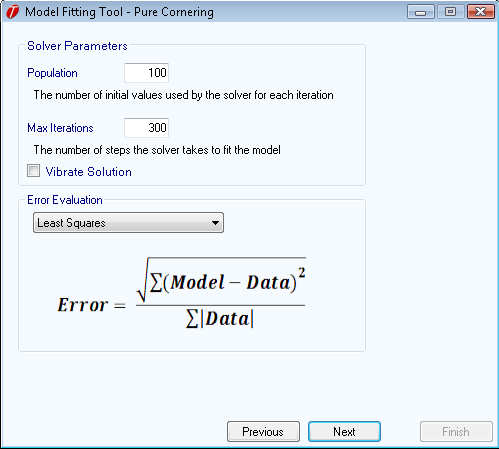
\includegraphics[width=1.0\textwidth]{SolverParameters.png}
	\caption{Solver Parameters and Error Evaluation}
	\label{fig:SolverParameters}
\end{figure}

The \textsl{Vibrate Solution} option will cause a small random variation to be applied to the data at each step. This can help the solver converge towards a global minimum slightly faster. Statistically, the variation is applied equally in both direction, so this technique does not bias the results.

The \textsl{Error Evaluation} can now be selected. This determines what type of error criteria is used when fitting the model. The four types of error criteria included in OptimumTire are described below. In the equations \textsl{Model} represents the value found by the model fitter and \textsl{Data} represents the value of the actual raw data.

\begin{itemize}
\item Least Squares Error:
\begin{displaymath}
Error=\frac{\sqrt{\sum\left(Model-Data\right)^2}}{\sum\left|Data\right|}
\end{displaymath}

\item	Normalized Least Squares Error:
\begin{displaymath}
Error=\frac{\sqrt{\sum\left(\frac{Model-Data}{Data}\right)^2}}{\# of data points}
\end{displaymath}

\item	Total Error:
\begin{displaymath}
Error=\frac{\sum\left|Model-Data\right|}{\sum\left|Data\right|}
\end{displaymath}

\item	Normalized Total Error:
\begin{displaymath}
Error= \frac{\sum\left|\frac{Model-Data}{Data}\right|}{\# of data points}
\end{displaymath}
\end{itemize}

Typically the \textsl{Least Squares Error} criteria will result in the best overall model fit. However depending on the variance and testing conditions of the raw data some of the other error criteria may produce a better fit. For example when fitting an aligning torque model \textsl{Total Error} will often produce slightly better results. The \textsl{Normalized Error} criteria gives equal weight to all of the data points. Therefore it will improve the model fitting at lower loads.

In the case that a weighting function is used, the error evaluation is modified to be the following. The weightin is denoted as $w_i$ and is evaluated for each data point separately.

\begin{itemize}
\item Least Squares Error:
\begin{displaymath}
Error=\frac{\sqrt{\sum w_i \left(Model-Data\right)^2}}{\sum\left|Data\right|}
\end{displaymath}

\item	Normalized Least Squares Error:
\begin{displaymath}
Error=\frac{\sqrt{\sum w_i \left(\frac{Model-Data}{Data}\right)^2}}{\# of data points}
\end{displaymath}

\item	Total Error:
\begin{displaymath}
Error=\frac{\sum w_i \left|Model-Data\right|}{\sum\left|Data\right|}
\end{displaymath}

\item	Normalized Total Error:
\begin{displaymath}
Error= \frac{\sum w_i \left|\frac{Model-Data}{Data}\right|}{\# of data points}
\end{displaymath}
\end{itemize}


\subsection*{Model Fitting}
Now OptimumTire is ready to fit the tire model. However, if something is incorrect or the user would like to change some of the settings the \textsl{Previous} button can be used to go back to the previous windows. Alternatively, the \textsl{Model Fitting Tool} window can be closed and the model fitting restarted.

Clicking on the \textsl{Summary} button allows the user to check to make sure all of the solver settings are correct. It will show the model being fit, the raw data to be used, the error calculation method, the coefficient boundary, and the solver parameters selected.  To return to the \textsl{Model Fitting Tool} window just close the model summary. Once the model fitting is finished this information will be automatically transferred into OptimumTire and will be stored with the associated tire model in the models data entry form.

Clicking on the \textsl{Start} button in the upper right corner of the window will start the solver. Figure~\ref{fig:ModelFitting} shows this window after a fitting has been completed. The graph shows the convergence of the solution and the textbox shows the current error as the model is fitted. When the final solution is found click on the \textsl{Finish} button to return to the main screen of OptimumTire.

 \begin{figure}[H]
	\centering
		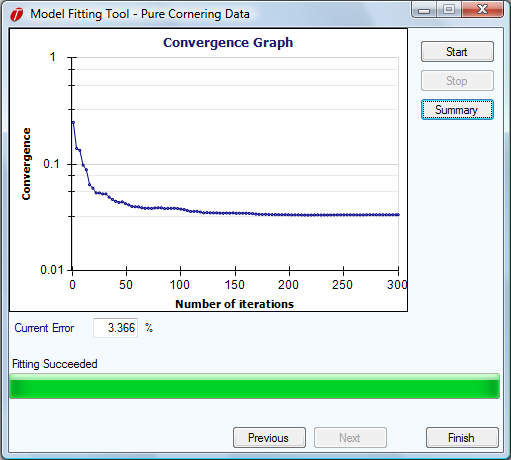
\includegraphics[width=1.0\textwidth]{ModelFitting.png}
	\caption{Model Fitting Convergence and Error}
	\label{fig:ModelFitting}
\end{figure}

The newly created tire model should now appear in the project tree. This model can now be graphed by selecting the check box next to it (Graphing is covered in Chapter~\ref{sec:AdditionalFeatures}). It should be compared to the raw data to ensure accuracy. Lateral force as a function of the slip angle at the tested inclination angles should be graphed and compared to the raw data as shown in Figure~\ref{fig:FySA}. Also the lateral force as a function of the normal load, Fz, for several slip angles should be graphed as in Figure~\ref{fig:FyFz}. The graphs should be checked for accuracy by comparing them with the raw data. The model should also be checked to ensure the curves are well behaved outside of the measurement area. This is especially important if the tire models are going to be used for simulation. Refer to section~\ref{sec:AdjustingModels} for information on adjusting the tire model.

 \begin{figure}[H]
	\centering
		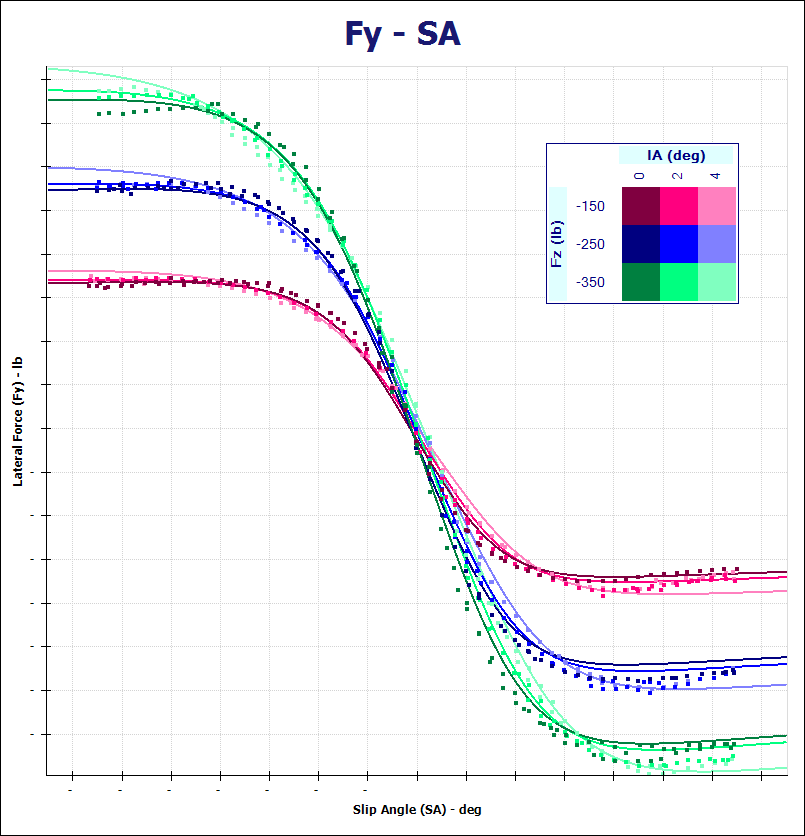
\includegraphics[width=1.0\textwidth]{FySA.png}
	\caption{Lateral Force vs. Slip Angle at Different Inclination Angles}
	\label{fig:FySA}
\end{figure}

 \begin{figure}[H]
	\centering
		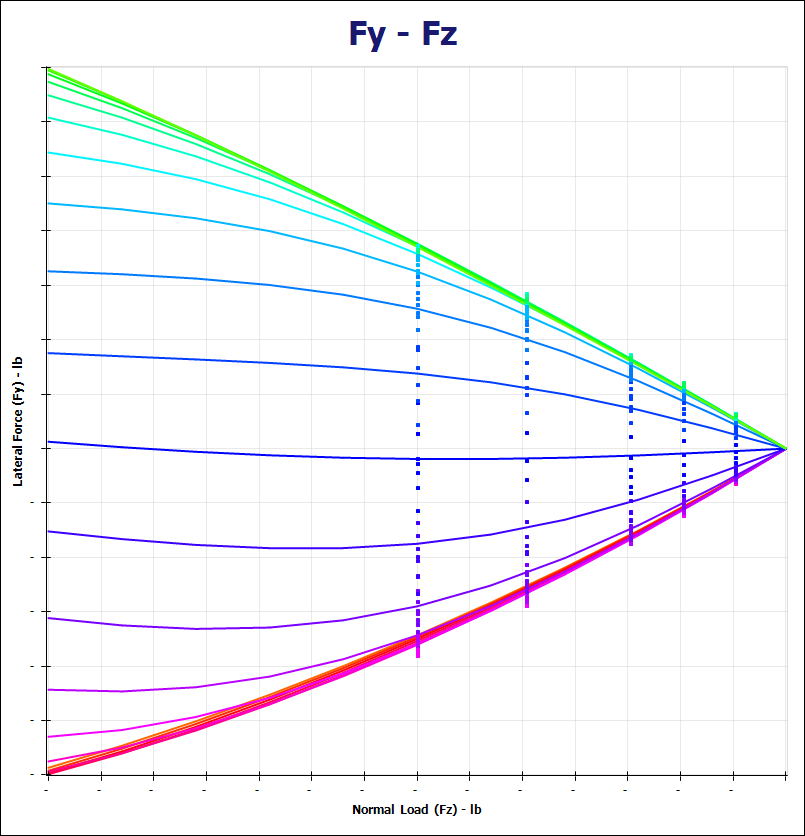
\includegraphics[width=1.0\textwidth]{FyFz.png}
	\caption{Lateral Force vs. Normal Load at Different Slip Angles}
	\label{fig:FyFz}
\end{figure}

\subsection{Aligning Torque Model}
\label{sec:AligningTorqueModel}
Fitting the aligning torque model is very similar to the lateral force model. However, there are a few small differences since this model will be combined with the lateral force model.

First select the tire data used to fit the lateral force model. In the \textsl{Model Fitting} section select the same type of tire model as was used for the lateral force model and click on the \textsl{Fit Model} button. This will open a different window than before since another tire model already exists in this project. Figure~\ref{fig:AdvancedFitting} shows the \textsl{Advanced Fitting Options} window.  In this window coefficients that were already determined in previously created models can be fixed for the current fitting. So for this example you would set the \textsl{Fy Pure} category to the previously created tire model. In later sections you will see that you can set multiple sets of coefficients and also include model scaling factors. Once the correct coefficients are selected click on the \textsl{Done} button.

 \begin{figure}[H]
	\centering
		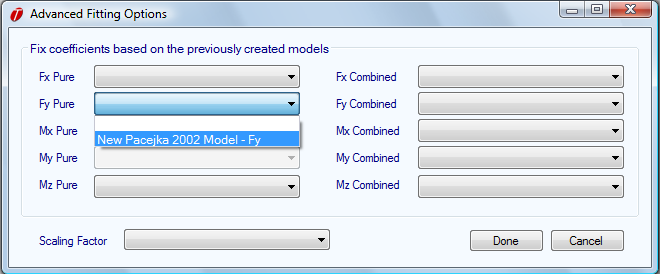
\includegraphics[width=1.0\textwidth]{AdvancedFitting.png}
	\caption{Advanced Fitting Options}
	\label{fig:AdvancedFitting}
\end{figure}

Now the \textsl{Model Fitting Selection} window that was used to fit the previous models will open. For this case \textsl{Calculate and Fit Error} in the drop down box labeled \textsl{Mz Pure} would be selected. As can be seen in Figure~\ref{fig:MzPureFit} the dropdown box corresponding to \textsl{Fy Pure} is disabled because the coefficients for this model were fixed in the previous step. The rest of the tire model can now be created in the same way as the lateral force model. When finished a new tire model will be created that contains both the pure lateral force and the aligning torque coefficients.
 
The aligning torque model could also have been created at the same time as the pure lateral force model, but for demonstration purposes was done separately. This would of have been achieved by selecting \textsl{Fit} or \textsl{Fit and Calculate Error} for both \textsl{Fy Pure} and \textsl{Mz Pure} when the coefficients to be fit were specified.
 The aligning torque as a function of the slip angle should be graphed with the tire data to check the accuracy of the model. An example of this is shown in Figure~\ref{fig:MzSA}.

 \begin{figure}[H]
	\centering
		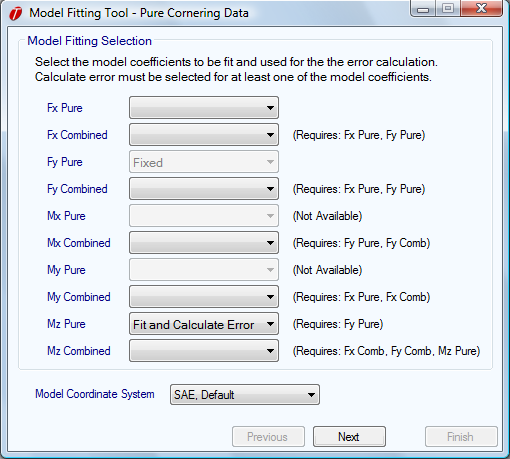
\includegraphics[width=1.0\textwidth]{MzPureFit.png}
	\caption{Specify Coefficients to be Fit}
	\label{fig:MzPureFit}
\end{figure}

 \begin{figure}[H]
	\centering
		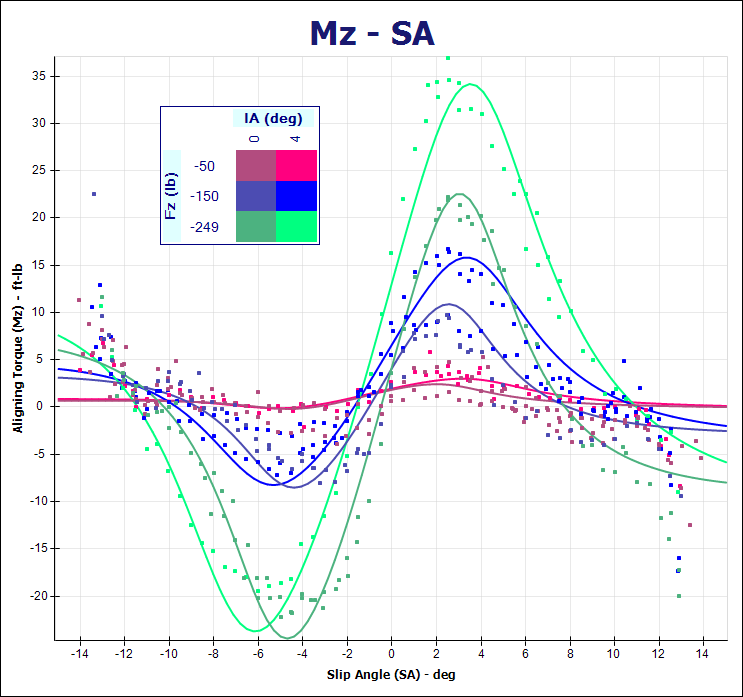
\includegraphics[width=1.0\textwidth]{MzSA.png}
	\caption{Aligning Torque vs. Slip Angle at Different Inclination Angles}
	\label{fig:MzSA}
\end{figure}

\label{sec:ModelScalingFactors}
\subsection{Model Scaling Factors}

In order to combine the data from a pure cornering test and a combined lateral and longitudinal test it will often be required to use a scaling factor.  It will adjust the pure lateral force model created from the cornering data to match the combined lateral and longitudinal data at zero slip ratio.

Figure~\ref{fig:UnscaledData} shows the discrepancy between the lateral force model and the combined data for the same tire. The pure lateral force model is represented by the solid lines and the combined data is the clusters of points at approximately 0, 3, and 6 degrees of slip angle. These points represent the force at zero slip ratio. This discrepancy is an effect of the pure cornering test being performed at a constant slip ratio and varying slip angle, while the combined test is performed at a constant slip angle with a varying slip ratio. These tests are also often performed at different speeds. Additionally, the tire will experience different heat cycling in these tests and therefore different results would be produced.

 \begin{figure}[H]
	\centering
		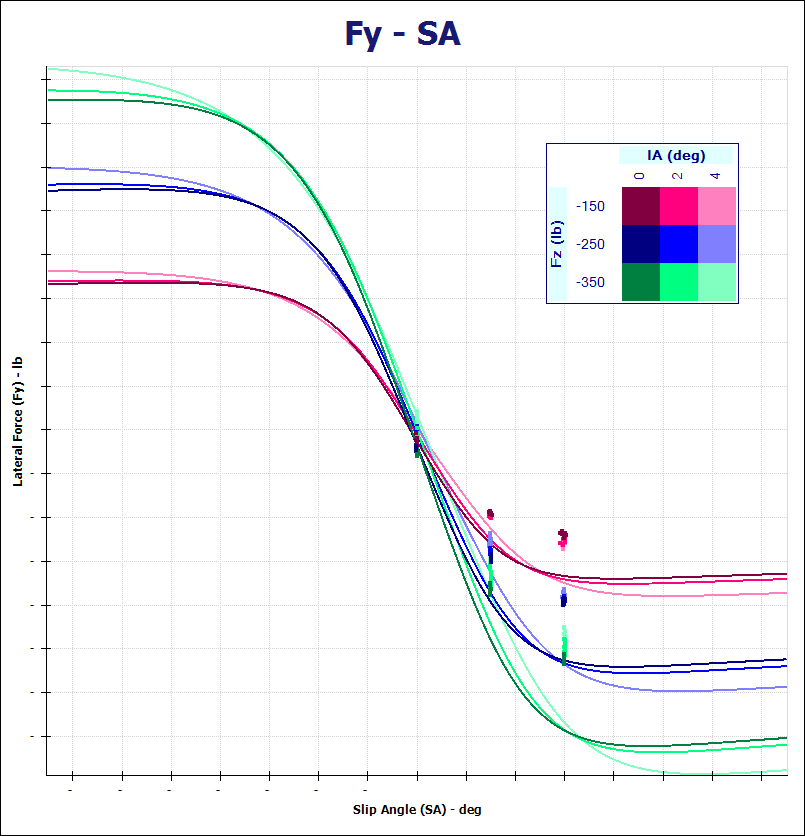
\includegraphics[width=1.0\textwidth]{UnscaledData.png}
	\caption{Lateral Force vs. Slip Angle for the Model and Data before Scaling}
	\label{fig:UnscaledData}
\end{figure}

Therefore to remedy this problem a scaling factor will be created and applied to the previously created models. To create a scaling factor click on the \textsl{New Scaling Factor} button in the upper right corner of the project tree area. Figure 3.16 shows this button, circled in red. Scaling factors can only be created for the Pacejka models. Similarly to the tire data and models, the scaling factor can be deleted, copied, or renamed by right clicking on it in the project tree.
 
In Figure~\ref{fig:NewScalingFactor} a previously added scaling factor can be seen in the project tree. The scaling factor can be applied to a tire model by dragging and dropping it onto the tire model or by right clicking on the tire model and choosing \textsl{Add Scaling Factor}. The small red "S" that appears on the selected tire model indicates that a scaling factor has been applied to the model. The scaling factor applied to a tire model can be removed or viewed by right clicking on the tire model.

 \begin{figure}[H]
	\centering
		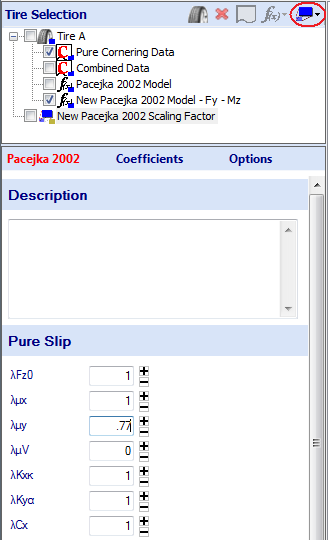
\includegraphics{NewScalingFactor.png}
	\caption{New Scaling Factor}
	\label{fig:NewScalingFactor}
\end{figure}

When a scaling factor is selected in the project tree its coefficients will appear in the data entry area as can also be seen in Figure~\ref{fig:NewScalingFactor}. A description of these coefficients appears in Table~\ref{tbl:PacejkaScalingCoefficients}. The coefficients can be modified manually or by double clicking on the "+" or "-". This will increase or decrease the value of the scaling factor by 10\%. If the scaling factor is applied to a graphed model holding down on these buttons will show a preview of the change (For more information on adjusting models refer to section~\ref{sec:AdjustingModels}). Decreasing the peak lateral friction coefficient, $\lambda\mu y$, will decrease the lateral force of the model. Figure~\ref{fig:ScaledModel} shows the lateral force of the model and data shown in Figure~\ref{fig:UnscaledData}.

 \begin{figure}[H]
	\centering
		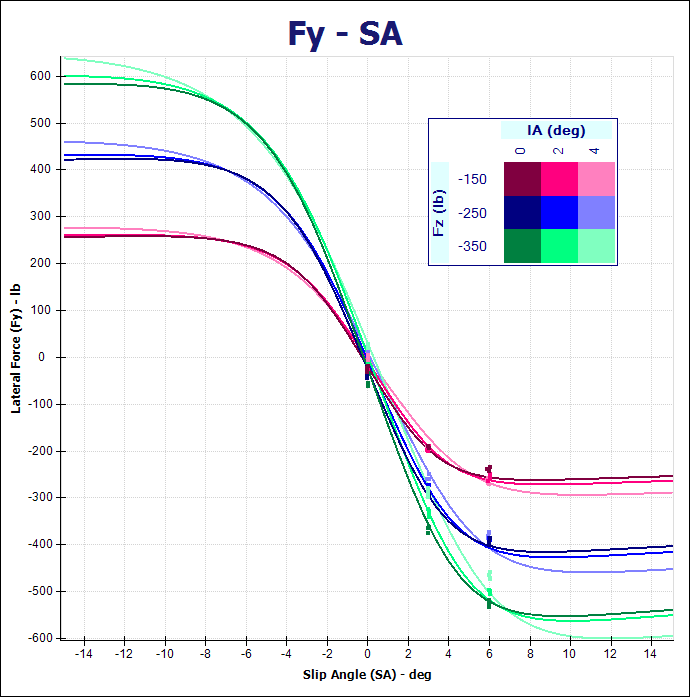
\includegraphics[width=1.0\textwidth]{ScaledModel.png}
	\caption{Lateral Force vs. Slip Angle for the Model and Data after Scaling}
	\label{fig:ScaledModel}
\end{figure}

Scaling factors are also commonly used to adjust tire models to more accurately represent the actual vehicle performance. This is necessary because the conditions and surfaces the tires are tested on are typically different than those they are to be used on. For more information regarding the scaling coefficients and their effect on the models please refer to the section~\ref{sec:PacejkaScalingFactors}.

\subsection{Pure and Combined Longitudinal Model}
\label{sec:PureandCombinedLongitudinalModel}
Now that the previously created model is properly scaled a pure longitudinal and combined longitudinal model can be created. This process will be similar to the previous models but both models will be created simultaneously. They will be created at the same time because the combined lateral and longitudinal tire data is collected at various slip angles. Thus the tire data is representative of pure and combined longitudinal force.

First, the combined data to be used should be imported and properly collapsed (These operations are covered in section~\ref{sec:RawTireData}). Then select the combined lateral and longitudinal tire data in the project tree. In the \textsl{Model Fitting} section select the appropriate tire model and click on the \textsl{Fit Model} button. This will open the \textsl{Advanced Fitting Options Window}. Set the dropdown boxes corresponding to \textsl{Fy Pure} and \textsl{Mz Pure} to the appropriate tire model to fix these coefficients. Click \textsl{Done} once this is completed.

The \textsl{Model Fitting Selection} window will now open. For this case you would select \textsl{Fit} in the \textsl{Fx Pure} drop down box and \textsl{Fit and Calculate Error} in the \textsl{Fx Combined} drop down box as shown in Figure~\ref{fig:MultipleModels}. You can also calculate the combined error for both models by selecting \textsl{Fit and Calculate Error} for both models. \textsl{Fit and Calculate Error} must be selected for at least one of the models. The rest of the tire model can now be created in the same way as the lateral force model. When finished a new tire model will be created that contains both the pure and combined longitudinal force coefficients.

 \begin{figure}[H]
	\centering
		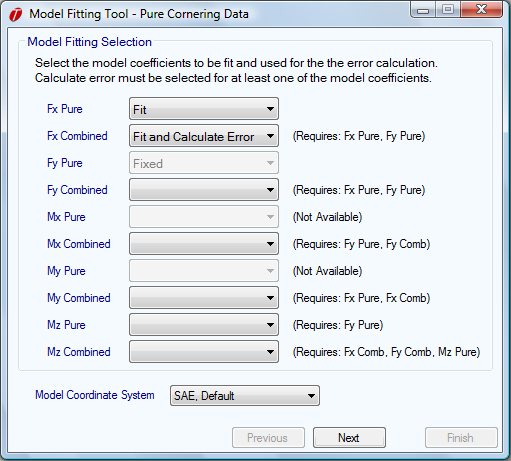
\includegraphics[width=1.0\textwidth]{MultipleModels.png}
	\caption{Fitting Multiple Models Simultaneously}
	\label{fig:MultipleModels}
\end{figure}

This model should be checked by graphing the longitudinal force as a function of the slip ratio and as a function of the normal load, Fz. Examples of these graphs are shown in Figure~\ref{fig:FxSR} and Figure~\ref{fig:FxFz}. You should check that the model curves correlate well to the tire data and are well behaved outside of the measurement area especially if the tire model is going to be used for simulation. If the models need to be adjusted please refer to section~\ref{sec:AdjustingModels}.

 \begin{figure}[H]
	\centering
		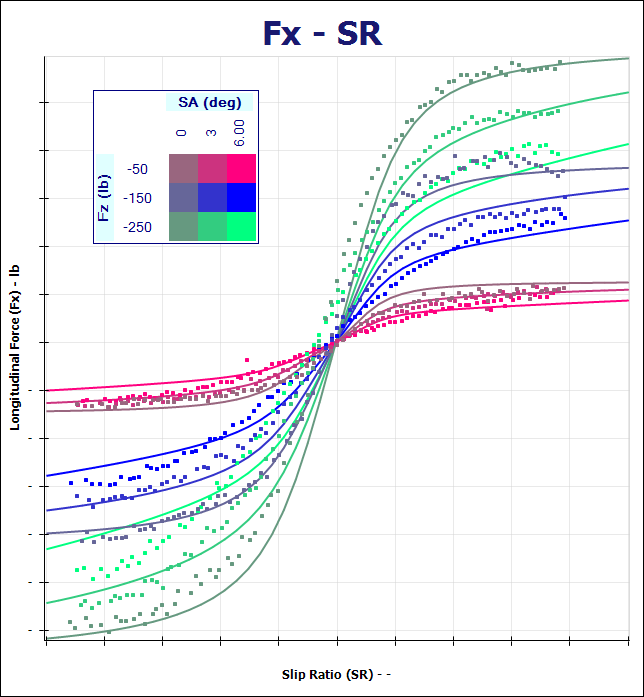
\includegraphics[width=1.0\textwidth]{FxSR.png}
	\caption{Longitudinal Force vs. Slip Angle at Different Slip Angles}
	\label{fig:FxSR}
\end{figure}

\begin{figure}[H]
	\centering
		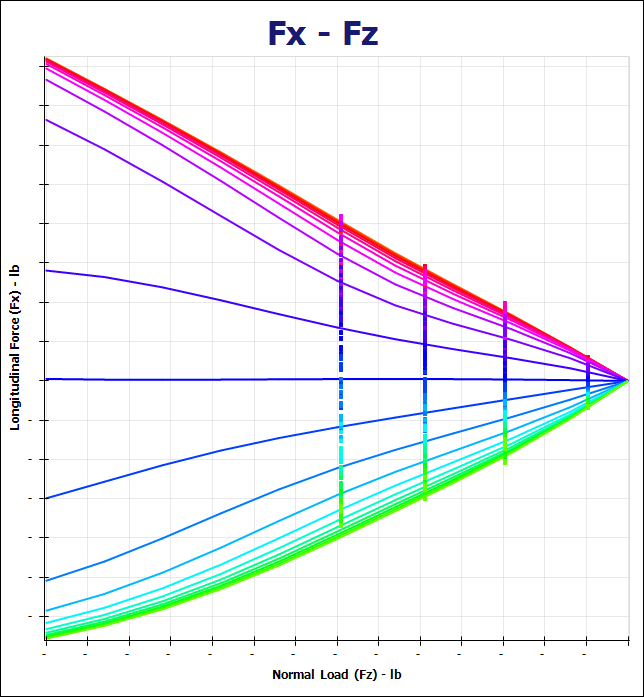
\includegraphics[width=1.0\textwidth]{FxFz.png}
	\caption{Longitudinal Force vs. Normal Load at Different Slip Ratios}
	\label{fig:FxFz}
\end{figure}

\subsection{Combined Lateral Model}
\label{sec:CombinedLateralModel}
The combined lateral model is also fit from the combined lateral and longitudinal data. The procedure is very similar to the other models except that the scaling factor should be applied when the model is fit. This is the case because the model will be based on the unscaled Fy Pure coefficients. This is done by selecting the appropriate scaling factor in the \textsl{Advanced Fitting Options} as is shown in Figure~\ref{fig:FittingwithScalingFactor}. As can also be seen in the figure all of the previously determined coefficients are set to the appropriate tire model.

\begin{figure}[H]
	\centering
		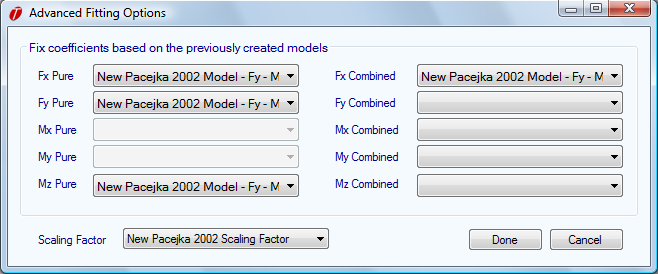
\includegraphics[width=1.0\textwidth]{FittingwithScalingFactor.png}
	\caption{Fitting with a Scaling Factor}
	\label{fig:FittingwithScalingFactor}
\end{figure}

A friction ellipse can now be plotted to ensure the accuracy of the combined lateral and longitudinal models. A graph of a friction ellipse is shown in Figure~\ref{fig:FrictionEllipse}. If these models are to be used for simulation it is very important to check that the model curves are well behaved outside of the measurement area.

\begin{figure}[H]
	\centering
		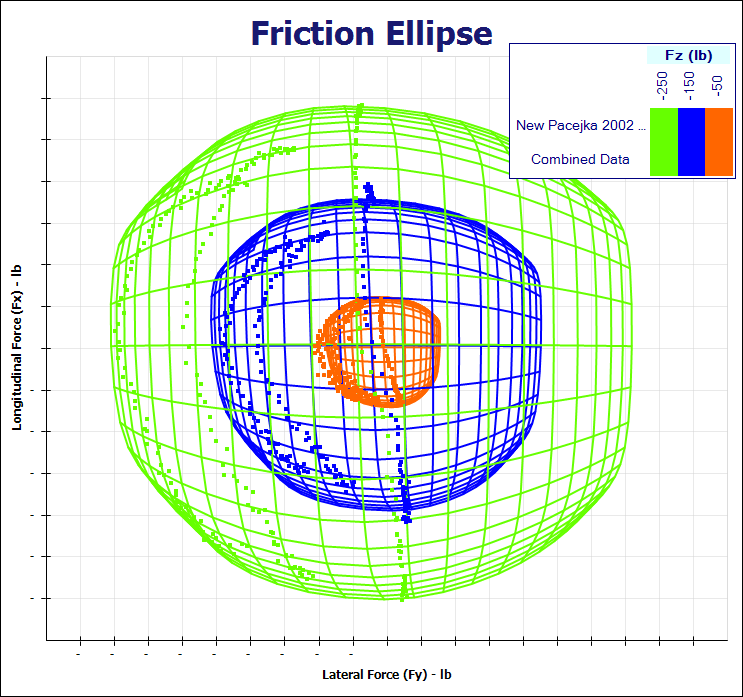
\includegraphics[width=1.0\textwidth]{FrictionEllipse.png}
	\caption{Friction Ellipse}
	\label{fig:FrictionEllipse}
\end{figure}

\subsection{Additional Models}
\label{sec:AdditionalModels}
Additional tire properties can also be fitted to the Pacejka models. These include combined models of aligning torque, rolling resistance, and overturning moment. Table~\ref{tbl:PacejkaModels} summarizes all of the models that can be fit to Pacejka coefficients in OptimumTire. It also shows what models are required before creating a new model. The required models can either be fixed prior to or fit concurrently with the new model. These models are fit in the same way as the previous example.

Table~\ref{tbl:PacejkaModels} displays the separate sets of coefficients that are available in the Pacejka models. Only combined, pure, rolling resistance and overturning models can be fit with the Pacejka models. The overturning moment and rolling resistance models are not available in the Pacejka '96 model.

\begin{table} [H]
	\centering
			\begin{tabular}{|l|l|l|}
			\hline
			\multicolumn{2}{|c|}{\cellcolor{tblue}\textbf{Model}} & \multicolumn{1}{|c|}{\cellcolor{tblue}\textbf{Requires}}\\ \hline
			Fx Pure &Longitudinal Force& \\ \hline
			Fx Comb	&Combined Longitudinal Force	&Fx Pure, Fy Pure\\ \hline
			Fy Pure	&Lateral Force& \\ \hline
			Fy Comb	&Combined Lateral Force	&Fx Pure, Fy Pure\\ \hline
			Mx Pure	&Overturning Moment	&Not Available\\ \hline
			Mx Comb	&Combined Overturning Moment	&Fx Pure, Fx Comb (not available in '96)\\ \hline
			My Pure	&Rolling Resistance	&Not Available\\ \hline
			My Comb	&Combined Rolling Resistance	&Fy Pure, Fy Comb (not available in '96)\\ \hline
			Mz Pure	&Aligning Torque	&Fy Pure\\ \hline
			Mz Comb	&Combined Aligning Torque	&Fx Comb, Fy Comb, Mz Pure\\ \hline
		\end{tabular}
	\caption{Pacejka Models (Mx Comb and My Comb are not available in the Pacejka �96 model)}
	\label{tbl:PacejkaModels}
\end{table}

\section{Model Fitting Order}
\label{sec:ModelFittingOrder}
The order in which the models are fit can vary depending on the tire data available and the goals of the project. However, since some of the models are dependent on each other there are some restrictions on the order. Table~\ref{tbl:PacejkaModels}, above, shows what models are required before other models can be fit. This is also displayed in the \textsl{Model Fitting Selection} window in OptimumTire. These requirements, which will vary depending on the type of model being fit, can be seen to the right of the dropdown boxes in Figure~\ref{fig:ModelFittingRequirements}. 

\begin{figure}[H]
	\centering
		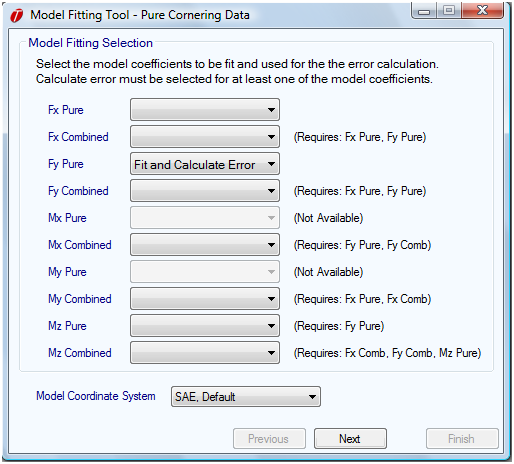
\includegraphics[width=1.0\textwidth]{ModelFittingRequirements.png}
	\caption{Model Fitting Requirements}
	\label{fig:ModelFittingRequirements}
\end{figure}

The two most common model fitting sequences will be described in Table~\ref{tbl:ModelFittingOrder} and Table~\ref{tbl:ModelFittingOrder2}. The first sequence uses pure lateral and combined data like the model fitting example in the previous sections. The second sequence uses pure lateral, pure longitudinal and combined data.
Under \textsl{Coefficients to be Fixed} the "Fix" indicates that these coefficients should be selected in the Advanced Fitting Options window. Under Coefficients to be Fit the "FE" indicates that these coefficients should be set to \textsl{Fit and Calculate Error} and the "Fit" indicates that these coefficients should be set to \textsl{Fit} in the \textsl{Model Fitting Selection} window.

\begin{table} [H]
	\centering
			\begin{tabular}{|c|c|c|c|c|c|c|c|c|c|c|c|c|c|}
			\hline
			\multicolumn{14}{|c|}{\cellcolor{tblue}\textbf{Model Fitting with Pure Lateral and Combined Data}} \\ \hline
			\multirow{3}{*}{Step} & \multirow{3}{*}{Data Used} & \multicolumn{6}{|c|}{\cellcolor{ttblue}Coefficients to be Fixed} & \multicolumn{6}{|c|}{\cellcolor{ttblue}Coefficients to be Fit} \\ \cline{3-14}
			 & &\multicolumn{3}{|c|}{Pure}&\multicolumn{3}{|c|}{Combined}&\multicolumn{3}{|c|}{Pure}&\multicolumn{3}{|c|}{Combined} \\ \cline{3-14}
			 & &Fx	&Fy	&Mz	&Fx	&Fy	&Mz	&Fx	&Fy	&Mz	&Fx	&Fy	&Mz \\ \hline
			 1 & Pure Lat. & & & & & & & &Fe& & & & \\ \hline
			 2 & Pure Lat. & & Fix& & & & & &&Fe & & & \\ \hline
			 5 & Combined. & & Fix&Fix & & & &Fit  & & &Fe & & \\ \hline
			 4 & Combined. &Fix & Fix&Fix &Fix & & & & & & &Fe & \\ \hline
			 5 & Combined. &Fix & Fix&Fix &Fix &Fix & & & & & & &Fe \\ \hline
		\end{tabular}
	\caption{Model Fitting Order with Pure Lateral and Combined Data}
	\label{tbl:ModelFittingOrder}
\end{table}

\begin{table} [H]
	\centering
			\begin{tabular}{|c|c|c|c|c|c|c|c|c|c|c|c|c|c|}
			\hline
			\multicolumn{14}{|c|}{\cellcolor{tblue}\textbf{Model Fitting with Pure Lateral, Pure Longitudinal and Combined Data}} \\ \hline
			\multirow{3}{*}{Step} & \multirow{3}{*}{Data Used} & \multicolumn{6}{|c|}{\cellcolor{ttblue}Coefficients to be Fixed} & \multicolumn{6}{|c|}{\cellcolor{ttblue}Coefficients to be Fit} \\ \cline{3-14}
			 & &\multicolumn{3}{|c|}{Pure}&\multicolumn{3}{|c|}{Combined}&\multicolumn{3}{|c|}{Pure}&\multicolumn{3}{|c|}{Combined} \\ \cline{3-14}
			 & &Fx	&Fy	&Mz	&Fx	&Fy	&Mz	&Fx	&Fy	&Mz	&Fx	&Fy	&Mz \\ \hline
			 1 & Pure Lat. & & & & & & & &Fe& & & & \\ \hline
			 2 & Pure Lat. & & Fix& & & & & &&Fe & & & \\ \hline
			 5 & Combined. & & Fix&Fix & & & &Fit  & & &Fe & & \\ \hline
			 4 & Combined. &Fix & Fix&Fix & & & & & & & & & \\ \hline
			 5 & Combined. &Fix & Fix&Fix &Fix & & & & & & & & \\ \hline
			 6 & Combined. &Fix & Fix&Fix &Fix &Fix & & & & & & & \\ \hline
		\end{tabular}
	\caption{Model Fitting Order with Pure Lateral, Pure Longitudinal and Combined Data}
	\label{tbl:ModelFittingOrder2}
\end{table}

\section{Model Coefficient Form}
\label{sec:ModelCoefficientForm}
After a model is fit the coefficients corresponding to it can be accessed by clicking on the model in the tire project tree. This will display the model coefficient form in the data entry area as shown in Figure~\ref{fig:ModelCoefficientForm}. This form includes the model coefficients, a description box, and the option to change the name displayed in the legend for the model. In this form the model coefficients can be modified by the user. This will be covered in detail in the next section. 

\begin{figure}[H]
	\centering
		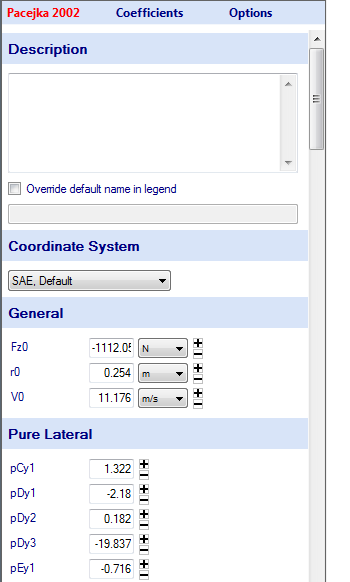
\includegraphics[height=0.6\textheight]{ModelCoefficientForm.png}
	\caption{Model Coefficient Form}
	\label{fig:ModelCoefficientForm}
\end{figure}

After a model is fit information regarding the model fitting will be directly imported into the description box as can be seen in Figure   The information included in the description box is the final error of the fitting, the model that was fit, the data file used, the coefficients fit, the error evaluation method, the coefficient boundary, and the solver parameters.

\section{Adjusting Models}
\label{sec:AdjustingModels}
Once the model is created and graphed against the raw data you might want to adjust it to improve its accuracy in a certain region or improve its behavior beyond the measurement area.  This can be done easily in OptimumTire.
  
Selecting a tire model in the project tree will show the model coefficients in the data entry area. You can modify the coefficients by 10\% by double clicking on the "+" or "-" button next to the coefficient \footnote[1]{When clicking the "+" and "-" button, the coefficient is either  multiplied or divided 1.10} . If the model is shown on a graph (see chapter~\ref{sec:AdditionalFeatures} for information about graphing), holding down the "+" or "-" button will show a preview of the model with the coefficient modified by 10\%. An example of this is shown in Figure~\ref{fig:ModelAdjustment}. In this figure the "+" button of the $pDy1$ coefficient is being held down. As can be seen in Figure~\ref{fig:ModelAdjustment} this change has a large effect on the graph. Changing other coefficients will have a much different effect on the curve both in terms of its magnitude and shape. The coefficients can also be adjusted manually by changing the values in the boxes. When applied to a tire model the coefficients of a scaling factor can be adjusted in the same way.

\begin{figure}[H]
	\centering
		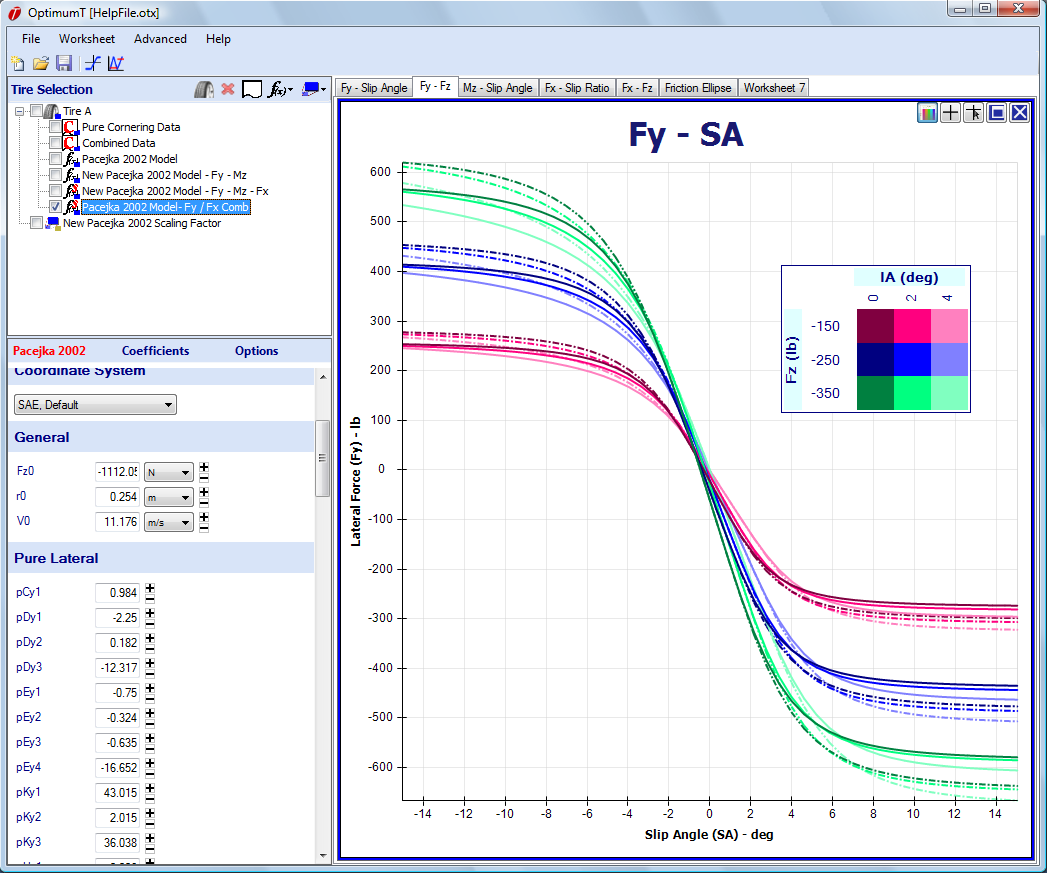
\includegraphics[width=1.0\textwidth]{ModelAdjustment.png}
	\caption{Model Adjustment Preview Feature}
	\label{fig:ModelAdjustment}
\end{figure}


\section{Creating Coefficient Boundaries From an Existing Model}
\label{sec:boundaryFromModel}

You can create a boundary from an existing model. When doing this, you specify the half-width of the boundary. In the model coefficient form, click on \textit{Options} then \textit{Create Boundary From Model} to arrive at the range specification (shown in Figure \ref{fig:BoundaryFromModel}). Enter the desired range and click the check-mark button. The minimum for each coefficient is created by reducing the the coefficient value by the user specified percentage, and the maximum is created by increasing the the value by the same amount. For example, if one of the coefficients of the model has a value or $1.00$ and you specify a boundary range of $10\%$, the minimum will be $0.90$ and the maximum will be $1.10$.

\begin{figure}
	\centering
		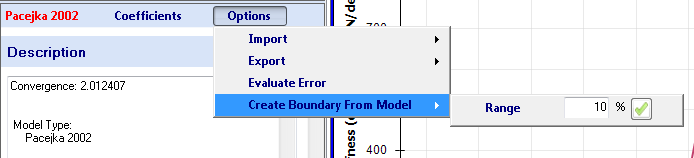
\includegraphics[width=0.80\textwidth]{BoundaryFromModel.png}
	\caption{Creating a boundary from an existing model.}
	\label{fig:BoundaryFromModel}
\end{figure}

Once you have clicked the check-mark button to create the boundary, you will be presented with the dialog shown in Figure \ref{fig:BoundaryFromModelSaveAs}. Enter the name to save the boundary as and choose a folder to put the boundary in.

\begin{figure}
	\centering
		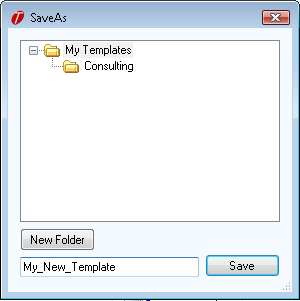
\includegraphics[width=0.40\textwidth]{BoundaryFromModelSaveAs.png}
	\caption{To save the boundary created from a model, specify the name to save it as in this dialog.}
	\label{fig:BoundaryFromModelSaveAs}
\end{figure}
